\subsection{Frameworks}


%1. I40 and IIC definition
%2. koloss industries clustering 
%3. what statistcs do we base our categorisation on
%4. where do you see yourself model (aka early adopter etc)

Both the industry and the academic world offer a variety of frameworks, concepts, consulting services and guidelines for businesses, institutions and even cities to employ to optimize their utility from the Digital Transformation.
We focused our attention on frameworks that are applicable to a variety of sectors to ensure we define recommendations applicable to businesses independent of region, industry or size. 
We chose three frameworks as applicable to most industries and want to summarize them in the following chapter.

\subsubsection{Industrie 4.0}
The German Industrie 4.0 initiative was created by the German government to improve Germanys economical position in the global market. According to the \emph{Plattform Industrie 4.0}, I4.0 is a specialization of the \emph{Internet of Things and Services} and applies to a subset of all industries, mainly focused on industrial production and manufacturing
\cite[p.41]{umsetzungsstrategie:2015}. Although it is specifically focused on the manufacturing sector, it is the most comprehensive initiative we found involving BITKOM e.V., VDMA e.V. and ZVEI e.V., three industrial associations representing IT, electronics and digital economy in Germany \cite{zveimembers:2016, vdmamembers:2016, bitkommembers:2016}. The initiative offers both recommendations and best practices for individual organizations \cite[p.40ff.]{umsetzungsstrategie:2015} as well as describing the strategic plan of progressing the \ac{I4.0} on a national level for the German government \cite[p.15ff.]{umsetzungsstrategie:2015}. It therefore offers a wide range of both high level overviews all the way do very detailed implementation advise on the factory floor.
 The following list summarizes the core goals. \footnote{It should be noted that only some of these goals are relevant to individual businesses trying to improve their strategy while others are global environmental necessities. Those that require action of individual businesses are marked with an (X).}

\begin{itemize}
	\item  Standardization (X)
	\item  Reducing of complexity (X)
	\item  Wideband infrastructure
	\item  Security (X)
	\item  Work culture and organization (X)
	\item  Education
	\item  Legal constraints (X)
	\item  Efficiency (X)
\end{itemize}
\cite[p.8]{umsetzungsstrategie:2015}
\footnote{The communcation infrastructure as well as education have been excluded under the assumption that they are inputs that are typically not produced by a business iteself but rather aquired externally.}

The I4.0 initiative offers several artifacts to support organizations in the transition to a digitalized organization as well as to facilitate the coordination between organizations and industries in researching and developing standards and technologies. 

The most prominent framework is \ac{RAMI} which has been created as a guideline to avoid definition of multiple, redundant and conflicting standards and communication strategies \cite[p. 41]{umsetzungsstrategie:2015}.

\begin{figure}[H]
\centering
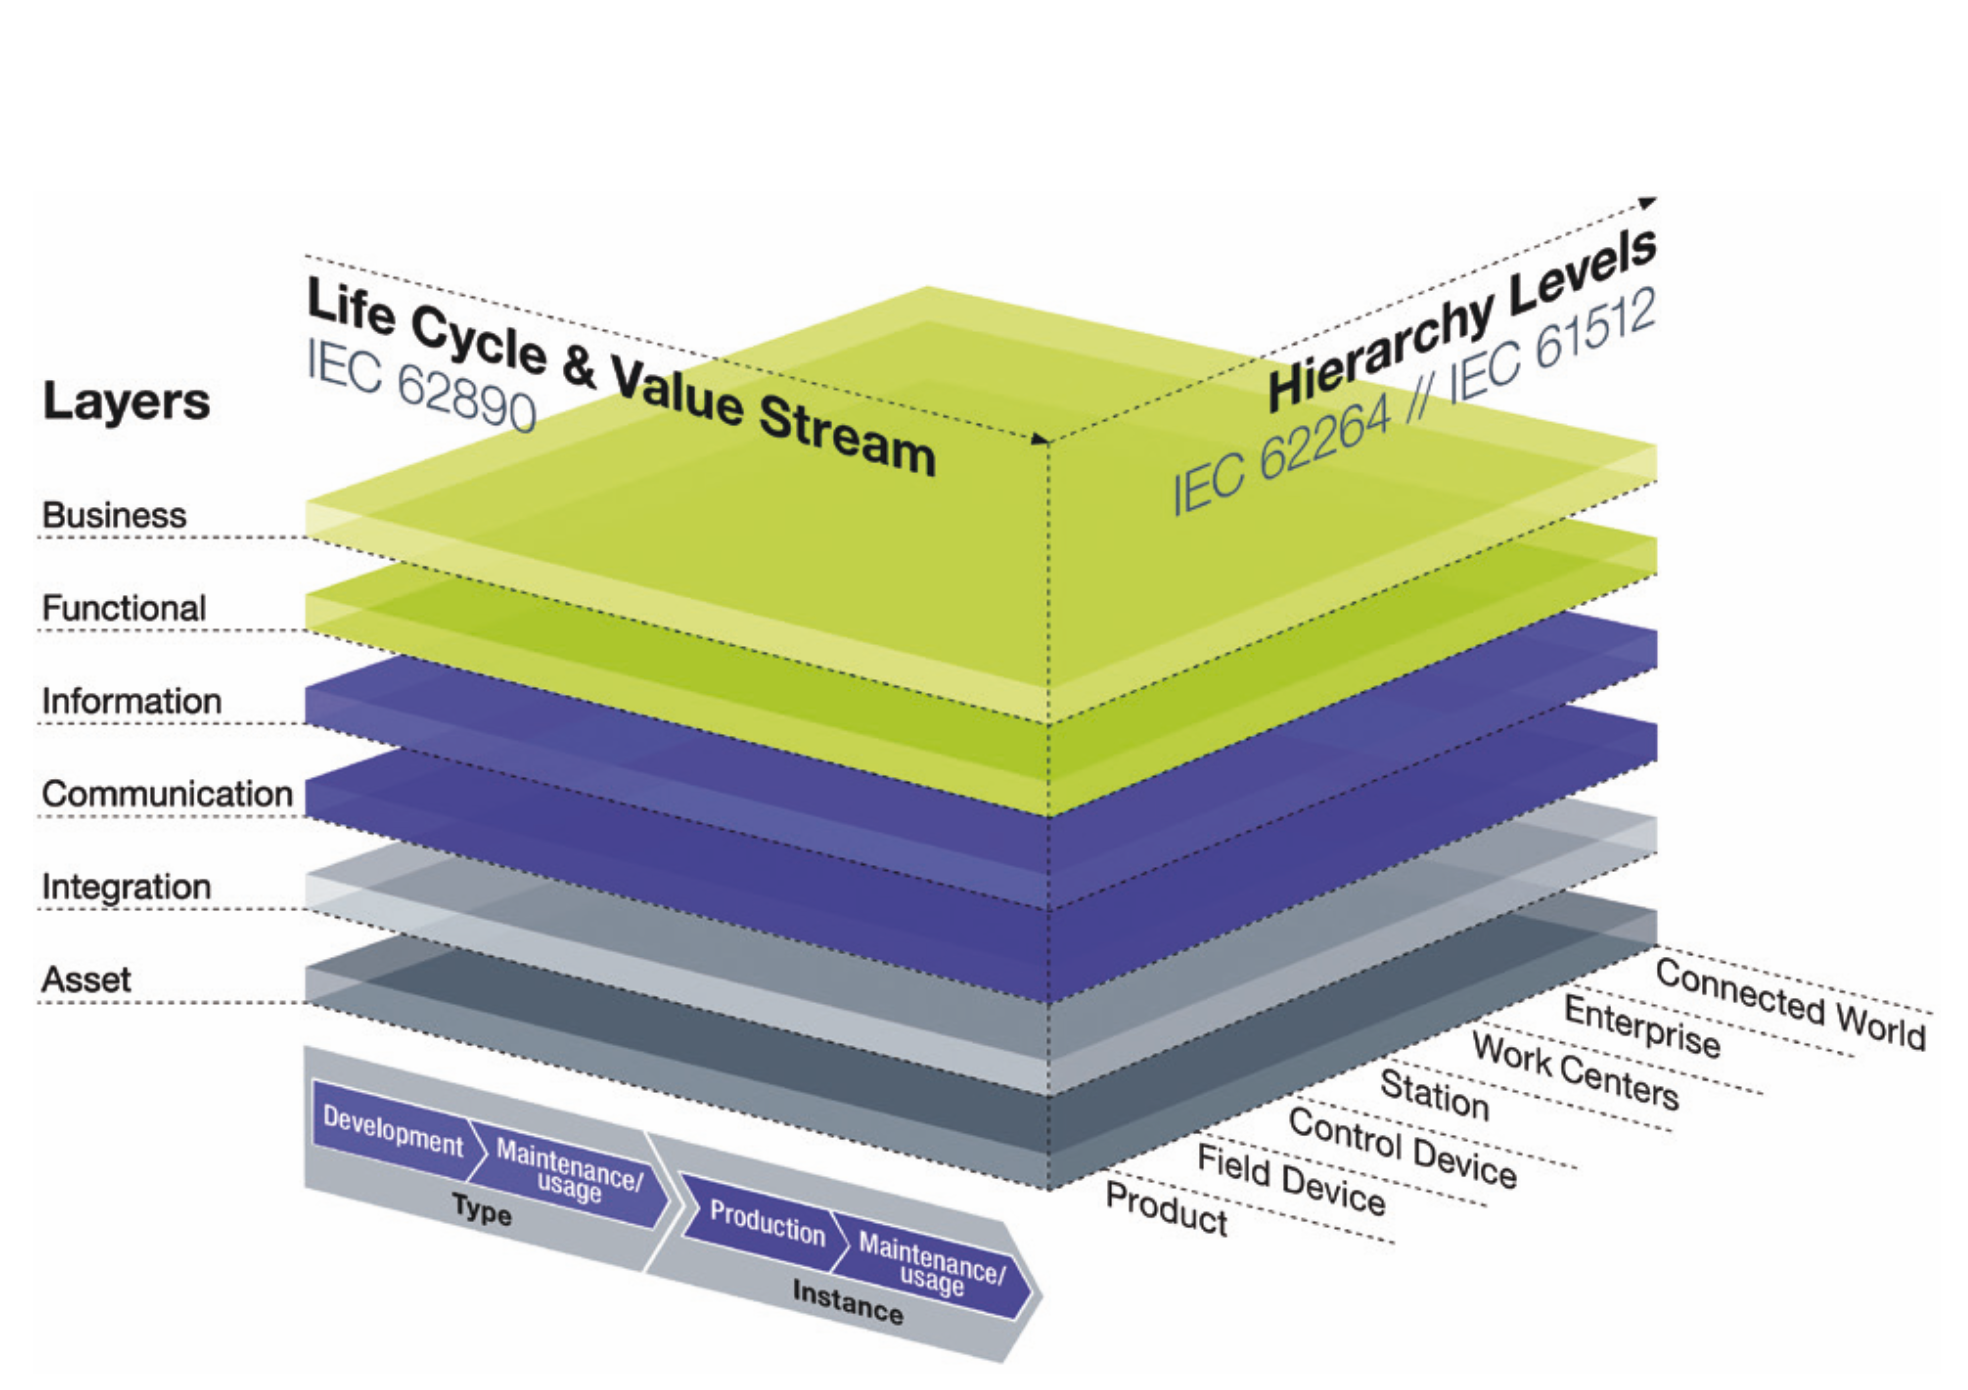
\includegraphics[width=1\columnwidth]{images/RAMI}
\caption{\ac{RAMI} from \cite{umsetzungsstrategie:2015}}
\end{figure}

The \ac{RAMI} framework focuses on three dimensions
%

\subsubsection{Industrial Internet Consortium}
The IIC is an 'open membership organization with 250 members from 30 countries, formed to accelerate the development, adoption and widespread use of interconnected machines and devices, intelligent analytics, and people at work'\cite{iic-progress:2016}. Its goals are as follows:

\begin{itemize}
	\item  Creation of use cases and testbeds
\item  Develop reference architectures and frameworks
\item  Influence the global development standards process
\item  Facilitate open forums
\item  Build confidence around approaches to security.
\end{itemize}
\cite{iic-aboutus:2016}


\subsubsection{Integrating IIC and I4.0}

Both the IIC and the I4.0 have announced collaboration efforts to ensure their goal of common standards and structures is achievable. While the IIC's efforts are targeted at a higher level of abstraction, the I4.0's focus is more narrow, focusing on the manufacturing and production industry. 


\begin{itemize}
	\item Business Model verification and redesign \cite{gassmann2013geschaeftsmodelle}
	\item Organizational Culture
	\item Technological capabilities and expertise
\end{itemize}




%\subsection{Terminology}

%\begin{itemize}
%\item
%what is Industrie 4.0 in relation to other words in the english-speaking environment
%\item
%does Industrie 4.0 also apply to industries that aren't involved in manufacturing
%\end{itemize}

%Compare to
%\cite{Wirtschaft_en:2016}
%and \cite{Wirtschaft:2016}
%for how the official translation handles the terms
